% --------------------
  \chapter{Pruebas en el COSMAC ELF II}
% --------------------
\label{C:pruebas_cosmac_elf_II}

%%%%%%%%%%%%%%%%%%%%%%%%%%%%%%%
En las instalaciones de la facultad de ingeniería se cuenta con el COSMAC ELF II, el cual fue comentado en la sección~\ref{C:cosmac_elf_II}. A modo de introducción, antes de comenzar a desarrollar los sistemas del proyecto, se realizaron pruebas sobre el COSMAC ELF II, para probar su funcionamiento y comenzar a comprender la operación del microprocesador. 

\begin{foto}[ht!]
  \centering
  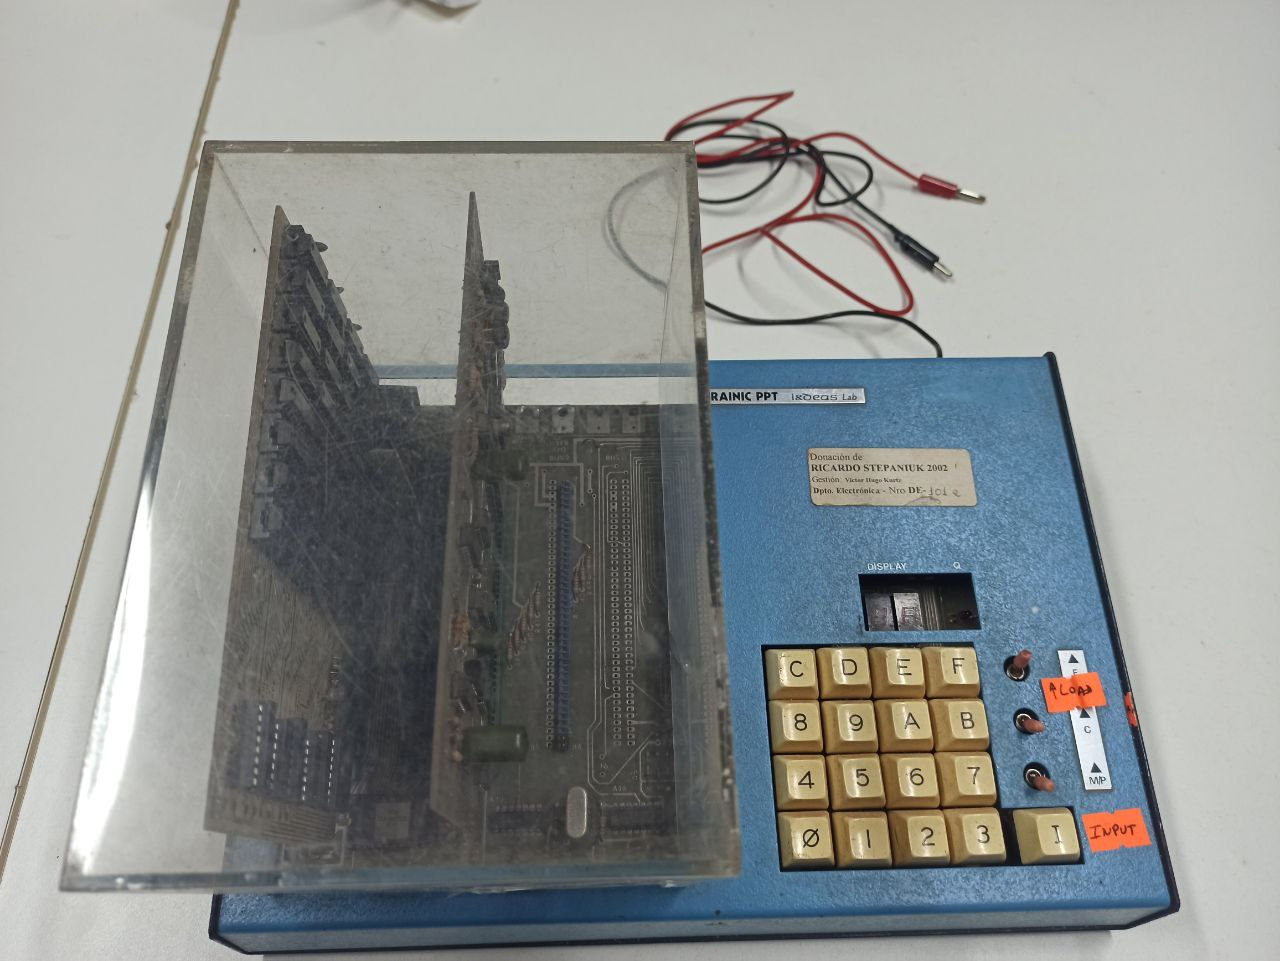
\includegraphics[width=.9\textwidth]{./imagenes/cosmac_elf_II_facu.jpg}
  \caption{COSMAC ELF II, propiedad de la facultad de ingeniería}
  \label{F:cosmac_elf_ii_falcultad}
\end{foto}

En la figura~\ref{F:cosmac_elf_ii_falcultad} se encuentra una fotografía del COSMAC ELF II que se encuentra en la facultad. Para utilizarlo fue necesario realizar reparaciones sobre el mismo. Un capacitor de entrada en la etapa de alimentación (en paralelo al pin de entrada del regulador LM7805) se encontraba dañado y fue necesario reemplazar el mismo, como así también soldar un cable a la placa para reemplazar una pista que se encontraba dañada. Luego se soldaron dos cables a los pines de alimentación de la placa de la computadora, para así poder conectarla a una fuente de alimentación.

Una vez realizadas estas reparaciones, se conectó el COSMAC ELF II a una fuente de alimentación configurada a \num{8}~\si{\volt} y se encendió. Para comprobar su funcionamiento correcto, se grabaron dos programas encontrados en línea \cite{programacion_cosmac}, junto con la explicación detallada del procedimiento para realizar la programación.

Se puede cargar un programa en el COSMAC ELF II poniendo el interruptor LOAD en la posición ON, con RUN y MP (Memory Protect) en OFF, y luego ingresar un byte con el teclado para finalmente presionar el botón INPUT. Esto graba un byte en la primera dirección de memoria. Para grabar otro byte en la siguiente dirección de memoria simplemente se debe ingresar el mismo en el teclado y volver a presionar INPUT. Una vez que se ingresaron todos los bytes del programa, MP debe colocarse en ON para proteger la memoria.

Con el programa ya cargado, para correrlo, se debe colocar LOAD en ON, esto resetea el microprocesador, luego se coloca RUN en ON, con lo cual el programa comienza a funcionar.

Siguiendo este procedimiento, se comprobó el funcionamiento del COSMAC ELF II con dos programas, uno que hace parpadear el LED Q, y otro que enciende el mismo cuando el botón INPUT es presionado.


%%%%%%%%%%%%%%%%%%%%%%%%%%%%%%%


